
\section{Matrices en vectoren in NumPy}
Om te kunnen werken met matrixes en vectoren gebruiken we in Python het package NumPy (\url{numpy.scipy.org}). Hoewel NumPy een datatype \textit{matrix} heeft, maak je voor het werken met matrices in de regel gebruik van een array van arrays (de klasse \textit{matrix} is deprecated en zal worden uitgefaseerd). Een NumPy-array is een homogene multidimensionale array: een verzameling van elementen van hetzelfde type. Het datatype van een NumPy-array is \texttt{ndarray}, wat iets anders is dan de standaard Python-array (die is namelijk 1-dimensionaal en heeft minder functionaliteit).

\subsection{Maken van matrices en vectoren}
De dimensionaliteit van een ndarray wordt uitgedrukt in \textit{assen} (\textit{axis}): een 2 \times 3 matrix wordt in een ndarray gerepresenteerd als een array van twee arrays (axis 1) met elk drie elementen (axis 2). Let op dat in NumPy arrays zero-based zijn, terwijl in de literatuur over lineaire algebra de verzamelingen meestal 1-based zijn. De dimensionaliteit van een ndarray kun je opvragen met de methode \textit{shape()}. Je kunt een matrix of vector transponeren met behulp van de \textit{property} \texttt{T}. De \href{https://docs.scipy.org/doc/numpy/reference/generated/numpy.array.html}{NumPy array API} definieert vijf parameters bij het aanmaken van een ndarray, waarvan alleen de eerste verplicht is: hierin zit de data waarvan een ndarray gemaakt moet worden. Zie de voorbeelden hieronder:

\begin{python}
import numpy as np
v1 = np.array([2,3,5,7])
v2 = np.array([[2,3,5,7],[2,4,6,8]])
v1.shape()
> (4,)
v2.shape()
(2,4)
v2.T.shape
> (4, 2)
\end{python}

In deze voorbeelden bevat \texttt{v1} een 1-dimensionale array, terwijl \texttt{v2} een 2-dimensionale array bevat – de data is dus feitelijk een array met twee elementen, beide een array van vier elementen: \texttt{v2} kun je dus beschouwen als een $2 \times 4$ matrix. Let ook op de \texttt{shape} van \texttt{v1}: waar je misschien (1,4) zou verwachten, krijg je (4,). Dit komt omdat we een tupel hebben aangemaakt met maar één element, namelijk de array [2,3,5,7]; deze notatie-vorm (met een 'leeg' tweede element) is de standaard Python manier om dergelijke tupels weer te geven. Dit kan problemen opleveren wanneer je deze array als vector wilt gebruiken (bijvoorbeeld wilt transponeren of vermenigvuldigen met een andere vector of een matrix). Er zijn verschillende mogelijkheden om dit punt te adresseren:

\begin{python}
np.array([[2,4,6,8]]).shape
> (1, 4)
np.array([1,3,5,7], ndmin=2).shape
> (1, 4)
\end{python}

Het benaderen van individuele elementen uit een vector of matrix gaat zoals je zou verwachten, met blokhaken en een \textit{zero-based} index. Je gebruikt een dubbele punt om ranges aan te geven. Als je alleen een dubbele punt gebruikt, krijg je de hele rij of kolom te zien. Zie de voorbeelden in de afbeelding hieronder. 

\begin{figure}[h]
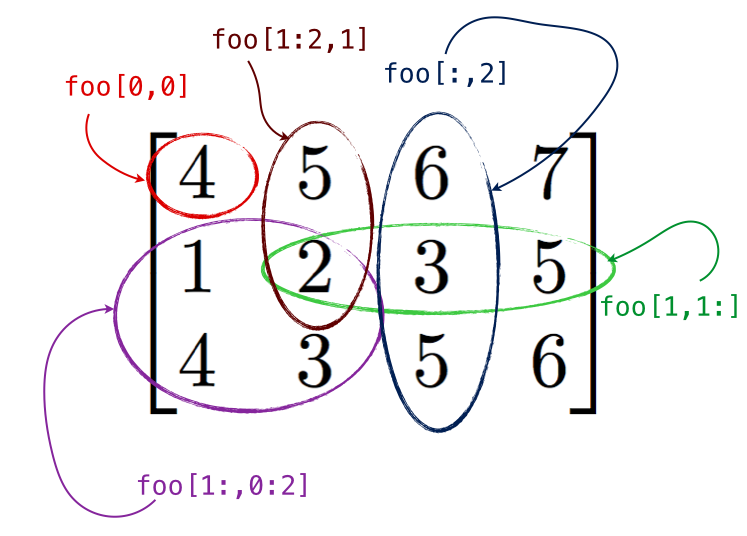
\includegraphics[width=.75\textwidth]{matrix1}
\centering
\end{figure}

Je kunt met NumPy ook eenvoudig een identiteitsmatrix maken, of een matrix van een bepaalde grootte gevuld met nullen, enen, of willekeurige getallen (tussen 0 en 1, of met een bepaalde range van gehele getallen):

\begin{python}
np.eye(3,4)         # identiteitsmatrix
np.zeros((2,3))     # nullen
np.ones((2,3))      # enen
np.random.rand(2,3) # random tussen 0 en 1
np.random.randint(5, size=(2,3))
\end{python}

Om een kolom of een regel aan een reeds bestaande matrix toe te voegen, zijn er verschillende mogelijkheden. Zo kun je bijvoorbeeld gebruik maken van de methoden \textit{\href{https://docs.scipy.org/doc/numpy/reference/generated/numpy.hstack.html}{hstack}} of \textit{\href{https://docs.scipy.org/doc/numpy/reference/generated/numpy.vstack.html}{vstack}}, je kunt negatieve kolommen of rijen van een bepaalde waarde voorzien, of je maakt gebruik van \texttt{c\_} of \texttt{r\_}. De afweging tussen de alternatieven zit hem vooral in de flexibiliteit versus de snelheid versus het geheugenverbruik. In de voorbeelden hieronder worden deze drie methoden gebruikt om een nieuwe matrix \texttt{X2} te maken, die gelijk is aan \texttt{X} met een extra kolom van enen aan de linkerkant hiervan – vergelijkbare technieken kun je gebruiken om regels toe te voegen. Ga er van uit dat \texttt{X}, \texttt{m} en \texttt{n} telkens weer zijn vernieuwd.


\begin{python}
X = np.random.randint(9, size=(8,6))
m,n = X.shape
>
#methode 1
foo = np.ones((m,1))
X2 = np.hstack((foo, X))
>
#methode 2
X2 = np.ones((m, n+1))
X2[:, 1:] = X
>
#methode 3
X2 = np.c_[np.ones(m), X]
\end{python}


\subsection{Omvormen, kopiëren en sorteren}
Stel je voor dat je een hele zooi data hebt die is opgeslagen als een $m \times n$ matrix – bijvoorbeeld een verzameling van 2-dimensionale plaatjes of reistijdentabellen. Soms wil je dergelijke data in één grote matrix representeren, bijvoorbeeld om deze in één keer op te kunnen slaan of alle data in één keer aan een bepaalde methode door te geven. In dat geval is het handig om de afzonderlijke matrices om te vormen in een $mn \times 1$ kolomvector of een $1 \times nm$ rijvector en deze vectoren in een grotere matrix op te slaan. We gebruiken hier de methode \textit{\href{https://docs.scipy.org/doc/numpy/reference/generated/numpy.resize.html}{resize}}: een methode die een array (of, dus, een matrix) een andere dimensionaliteit geeft. In het voorbeeld hieronder maken van we van twintig 8 \times 5 (willekeurige) matrices een grote 20 \times 40 matrix. Let op dat we de data eerst aan een lijst toevoegen en daarna de gehele lijst in één keer aan de constructor van de array meegeven.

\begin{python}
foo = []
for _ in range(20):
    foo.append(np.random.randint(8, size=(8,5)))
newlist = []
for m in foo:
    newlist.append(np.resize(m, [1,40])[0])
X = np.array(newlist)
\end{python}

Als je twee instanties van dezelfde vector wilt hebben, moet je gebruik maken van de methode \href{https://docs.scipy.org/doc/numpy/reference/generated/numpy.copy.html}{copy}. Eenvoudig een tweede variabele gelijk stellen aan de eerste die naar de vector verwijst werkt niet, omdat je daarmee alleen de \textit{pointers} gelijk maakt.

\begin{python}
foo = np.array([ [2,3],[4,5] ])
bar = foo
bar[0][0] = 9
foo
> array([[9, 3],
>       [4, 5]])
#terwijl
foo = np.array([ [2,3],[4,5] ])
bar = np.copy(foo)
bar[0][0]=9
bar
> array([[9, 3],
>       [4, 5]])
foo
> array([[2, 3],
>       [4, 5]])

\end{python}

Om arrays te sorteren gebruik je de methode \textit{\href{https://docs.scipy.org/doc/numpy/reference/generated/numpy.sort.html}{sort}}. Omdat een matrix ook een vector is, kun je deze methode ook gebruiken om matrices te sorteren. Het is dan wel van belang dat je aangeeft langs welke as (axis) je de matrix wilt sorteren: je kunt immers de \textit{kolommen} of de \textit{rijen} sorteren, zoals in het voorbeeld hieronder: 

\[
\begin{aligned}
X &=
\begin{bmatrix}
2 & 3 & 4 \\
5 & 7 & 1 \\
\end{bmatrix},\\
X_{hor} &=
\begin{bmatrix}
2 & 3 & 4 \\
1 & 5 & 7 \\
\end{bmatrix},\\
X_{ver} &=
\begin{bmatrix}
2 & 3 & 1\\
5 & 7 & 4\\
\end{bmatrix}.
\end{aligned}
\]

In NumPy bereik je dit effect als volgt:

\begin{python}
X = np.array([ [2,3,4],[5,7,1] ])
np.sort(X, axis=-1) #default waarde voor axis
array([[2, 3, 4],
       [1, 5, 7]])
np.sort(X, axis=0)
array([[2, 3, 1],
       [5, 7, 4]])

\end{python}

\subsection{Rekenen met matrices en vectoren}
Je kunt gebruik maken van de gewone wiskundige operatoren in Python om berekeningen op vectoren uit te voeren. Standaard werken deze operatoren per element (\textit{element wise}). Dat heeft tot gevolg dat als je een gewone operator gebruikt om twee matrices op te tellen of te vermenigvuldigen, deze dezelfde dimensionaliteit moeten hebben (elk element uit de linkermatrix moet gekoppeld kunnen worden uit een element uit de rechter).

\begin{python}
foo = np.array([ [2,3,5], [1,3,7] ])
bar = np.array([ [4,5,6], [1,2,3] ])
foo + bar
> array([[ 6,  8, 11],
>       [ 2,  5, 10]])
foo - bar
> array([[-2, -2, -1],
>       [ 0,  1,  4]])
foo*2
> array([[ 4,  6, 10],
>       [ 2,  6, 14]])
foo**2
> array([[ 4,  9, 25],
>       [ 1,  9, 49]])
foo+2
> array([[4, 5, 7],
>       [3, 5, 9]])
\end{python}

Wanneer we twee matrices niet \textit{element wise} met elkaar willen vermenigvuldigen, maar op de manier zoals dat bij de lineaire algebra is beschreven, moeten we gebruik maken van de NumPy-methode \href{https://docs.scipy.org/doc/numpy/reference/generated/numpy.matmul.html#numpy.matmul}{matmul} (of, wat op hetzelfde neerkomt, \texttt{a @ b}) – let dan wel op de correcte dimensionaliteit van de matrices. Wanneer we twee vectoren met elkaar willen vermenigvuldigen, kunnen we gebruik maken van \textit{\href{https://docs.scipy.org/doc/numpy/reference/generated/numpy.dot.html}{dot}}.

\begin{python}
#twee matrices
X1 = np.array([ [2,3,5], [1,3,7] ])
X2 = np.array([ [4,5], [1,2], [5,6] ])
X1 @ X2
> array([[36, 46],
>       [42, 53]])
#maar
foo = np.random.randint(5, size=(2,3))
bar = np.random.randint(6, size=(4,5))
foo@bar
> Traceback (most recent call last):
>  File "<stdin>", line 1, in <module>
>  ValueError: shapes (2,3) and (4,5) not aligned: 3 (dim 1) != 4 (dim 0)
#twee vectoren
foo = np.array([2,3,4])
bar = np.array([6,7,8])
foo.dot(bar)
> 65
\end{python}
